Der Versuch besteht aus zwei Teilen. Zunächst wird ein Acrylblock mit Unregelmäßigkeiten untersucht. Die eingebohrten Löcher mit unterschiedlichem Radius sind wie in Abbildung \ref{fig:acrylblock} nummeriert. Die Struktur des Blockes wird sowohl mit einem A-Scan als auch mit einem B-Scan von beiden Längsseiten untersucht. \\
Im zweiten Versuchsteil wird ein die Bewegung eines Herzens simuliert und mit einem TM-Scan aufgenommen. Das Herzmodell bestehlt aus einem Zylinder der zu einem Drittel mit Wasser gefüllt ist. Der Zylinderboden ist eine Membran, die per handbetriebener Pumpe auf und ab bewegt wird. 
\todo[color=red]{Hast du ein anderes Wort für "Handpumpe"?}
\todo[color=green]{Vielleicht "handbetriebene Luftpumpe"?}


\begin{figure}[h!]
	\centering
	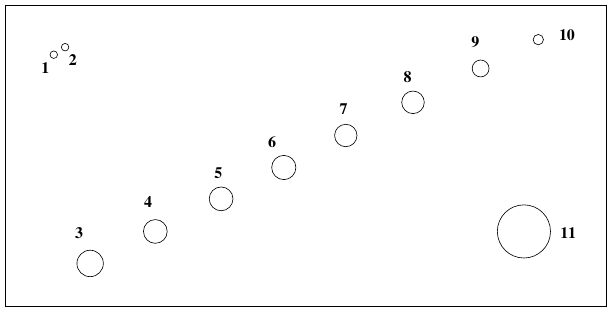
\includegraphics[width=0.7\textwidth]{Acrylblock.png}
	\caption{Nummerierung der Löcher im Acrylblock}
	\label{fig:acrylblock}
\end{figure}
